% Data flow diagram
% Author: David Fokkema
\documentclass{article}
\usepackage{tikz}
\usetikzlibrary{shapes,arrows}
\usepackage{pdflscape}
\usepackage[papersize={7.1cm, 7cm}, text={7.1cm, 7cm}]{geometry}
\usetikzlibrary{decorations.text}
\usepackage{xcolor}
% \selectcolormodel{gray}

\begin{document}
\thispagestyle{empty}
%\begin{landscape}
\begin{center}
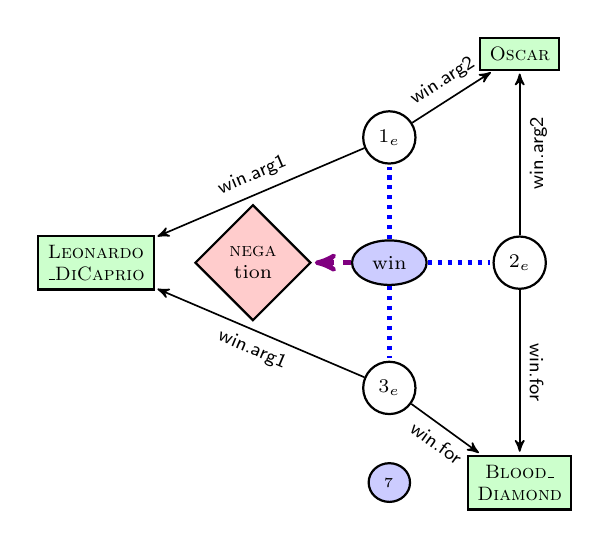
\begin{tikzpicture}[
  font=\sffamily,
  every matrix/.style={ampersand replacement=\&,column sep=0.5cm,row sep=0.5cm,font=\scriptsize},
  entity/.style={draw,thick,rectangle,fill=green!20,font=\sc\scriptsize},
  word/.style={draw,thick,ellipse,fill=blue!20},
  mediator/.style={draw,thick,circle},
  entityType/.style={draw,thick,rounded corners,fill=yellow!20,inner sep=.3cm},
  mathType/.style={draw,thick,diamond,fill=red!20,font=\scriptsize},
  mediatorToEntity/.style={->,>=stealth',shorten
>=1pt,semithick,black,sloped,above,font=\sffamily\scriptsize},
  typeToEntity/.style={->,>=stealth',shorten >=1pt,semithick,black,sloped,above,font=\sffamily\scriptsize},
  wordToEntity/.style={-,>=stealth',shorten >=1pt,ultra
thick,dotted,blue,sloped,above,font=\sffamily\scriptsize},
  entityToMath/.style={->,>=stealth',shorten >=1pt,ultra
thick,dashed,violet,sloped,above,font=\sffamily\scriptsize},
  every node/.style={align=center}]

  %  Leonardo DiCaprio did not win an Oscar for Blood Diamond .
  
  % Position the nodes using a matrix layout
  \matrix{ 
   \& \&  \& \node[entity] (eOscar) {Oscar}; \\
     \& \& \node[mediator] (m1) {1$_{e}$}; \&  \\
    \node[entity] (eDicaprio) {Leonardo\\\_DiCaprio}; \& \node[mathType] (mNeg) {\sc 
nega\\tion}; \& \node[word] (wWin)
{win}; \& \node[mediator] (m2) {2$_{e}$}; \\
   \&  \& \node[mediator] (m3) {3$_{e}$}; \&  \\
   \&  \& \node[word] (wDiamond) {$_7$}; \& \node[entity] (eDiamond) {Blood\_\\Diamond}; \\
  };
 
  % words to entities
  % \draw [wordToEntity] (wDicaprio) edge node {}  (eDicaprio);
  % \draw [wordToEntity] (wOscar) edge node {}  (eOscar);
  % \draw [wordToEntity] (wDiamond) edge node {}  (eDiamond);
  
  % event word to mediators
  \draw [wordToEntity] (wWin) edge node {}  (m1);
  \draw [wordToEntity] (wWin) edge node {}  (m2);
  \draw [wordToEntity] (wWin) edge node {}  (m3);
  
  % mediator to entities
  \draw [mediatorToEntity] (m1) edge node {win.arg1}  (eDicaprio);
  \draw [mediatorToEntity] (m1) edge node {win.arg2}  (eOscar);
  
  \draw [mediatorToEntity] (m2) edge node {win.for}  (eDiamond);
  \draw [mediatorToEntity] (m2) edge node[below] {win.arg2}  (eOscar);
  
  \draw [mediatorToEntity] (m3) edge node[below] {win.arg1}  (eDicaprio);
  \draw [mediatorToEntity] (m3) edge node[below] {win.for}  (eDiamond);
  
  \draw [entityToMath] (wWin) edge node {}  (mNeg);
  
\end{tikzpicture} 
\scriptsize $\mbox{NEGATION}(\mbox{win.arg1}(e, \textsc{Leonardo\_DiCaprio})\; \wedge
\mbox{win.arg2}(e, \textsc{Oscar}) \wedge
\mbox{win.for}(e, \textsc{Blood\_Diamond}))$
\end{center} 

% \end{landscape}

% \begin{tikzpicture}
% \node (One) at (-3,0) [shape=circle,draw] {$One$}; 
% \node (Two) at (3,0) [shape=circle,draw] {$Two$};
% \def\myshift#1{\raisebox{-2.5ex}}
% \draw [->,thick,postaction={decorate,decoration={text along path,text align=center,text={|\sffamily\myshift|Some more bent text}}}] (One) to [bend right=45]  (Two);
% \def\myshift#1{\raisebox{1ex}}
% \draw [->,thick,postaction={decorate,decoration={text along path,text align=center,text={|\sffamily\myshift|Some bent text}}}]      (One) to [bend left=45] (Two);
% \end{tikzpicture}


\end{document}
